% TEXINPUT=tikzuml-v*:$TEXINPUT pdflatex abrt.tex
\documentclass{article}
\usepackage[utf8]{inputenc}
\usepackage[english]{babel}
\usepackage[usenames,dvipsnames]{xcolor}
\usepackage{tikz}
\usetikzlibrary{arrows,shapes,mindmap,shadows,positioning}
\usepackage{hyperref}
\usepackage{fullpage}
\usepackage{graphicx}
\usepackage{fancybox}
\usepackage{tikz-uml}

% The document is based on
% a% template from project management book "A Guide to the Project Management Body of
% Knowledge" (PMBOK Guide).


\title{ABRT Project Document}
\author{Karel Klíč, Michal Toman, Miroslav Lichvár}

\begin{document}
\maketitle

ABRT is a set of technologies that collects and evaluates software
crashes coming from Linux operating system deployments.

This is a top-level project document for ABRT.

TODO: What is ABRT doing.

TODO: Purpose of ABRT.
% --- help users, developers, security to do their job\ldots

\cleardoublepage
\tableofcontents

\cleardoublepage
\section{Project Charter}

\subsection{Statement of Work}

business need, product scope, strategic plan

\subsection{Business case}

\subsubsection{Enterprise Client-Side Use Case 1}

\begin{tikzpicture}
\umlactor[x=-4,y=0]{End User}
\umlactor[x=6,y=0]{Support Portal}
\begin{umlsystem}[x=1,fill=red!10]{ABRT Client}
\umlusecase[x=0,y=2.4]{Send a $\mu$Report}
\umlusecase[x=0,y=0.8]{Read an Advice}
\umlusecase[x=0,y=-0.8]{Send a Full Report}
\umlusecase[x=0,y=-2.4]{Open a New Case}
\end{umlsystem}
\umlassoc{End User}{usecase-1}
\umlassoc{End User}{usecase-2}
\umlassoc{End User}{usecase-3}
\umlassoc{End User}{usecase-4}
\umlassoc{Support Portal}{usecase-1}
\umlassoc{Support Portal}{usecase-2}
\umlassoc{Support Portal}{usecase-3}
\umlassoc{Support Portal}{usecase-4}
\end{tikzpicture}

\subsubsection{Enterprise Client-Side Use Case 2}

\begin{tikzpicture}
\umlactor[x=-6,y=0]{End User}
\umlactor[x=10,y=0]{Administrator}
\umlactor[x=10,y=-3]{Support Portal}
\begin{umlsystem}[x=1,fill=red!10]{ABRT Server}
\umlusecase[x=-2,y=2,name=send microreport]{Send $\mu$Report}
\umlusecase[x=-2,y=-2,name=send full report]{Send Full Report}
\umlusecase[x=2,y=5,width=3cm,name=view problem trends]{View Problem Trends}
\umlusecase[x=2,y=3,name=view problem list]{View Problem List}
\umlusecase[x=2,y=1,width=3cm,name=view individual problems]{View Individual Problems}
\umlusecase[x=2,y=-1,width=3cm,name=submit problem to support portal]{Submit Problem to Support Portal}
\umlusecase[x=2,y=-3,width=3cm,name=read advice from support portal]{Read Advice from Support Portal}
\umlusecase[x=2,y=-5,width=3cm,name=open new case in support portal]{Open New Case in Support Portal}
\end{umlsystem}
\umlassoc{End User}{send microreport}
\umlassoc{End User}{send full report}
\umlassoc{Administrator}{view problem trends}
\umlassoc{Administrator}{view problem list}
\umlassoc{Administrator}{view individual problems}
\umlassoc{Administrator}{submit problem to support portal}
\umlassoc{Administrator}{read advice from support portal}
\umlassoc{Administrator}{open new case in support portal}
\umlassoc{Support Portal}{submit problem to support portal}
\umlassoc{Support Portal}{read advice from support portal}
\umlassoc{Support Portal}{open new case in support portal}
\end{tikzpicture}

\subsubsection{Enterprise  Support Use Case}

\begin{tikzpicture}
\umlactor[x=-4,y=0]{Support Portal}
\umlactor[x=10,y=-2]{Package Maintainer}
\umlactor[x=10,y=2]{QA Engineer}
\begin{umlsystem}[fill=red!10]{ABRT Server}
\umlusecase[x=0,y=4,name=save reports]{Save Reports}
\umlusecase[x=0,y=2,width=2.6cm,name=find report duplicates]{Find Report Duplicates}
\umlusecase[x=0,y=0,name=retrace coredump]{Retrace Coredump}
\umlusecase[x=0,y=-2,name=debug coredump]{Debug Coredump}
\umlusecase[x=0,y=-4,name=analyze backtrace]{Analyze Backtrace}
\end{umlsystem}
\umlassoc{Support Portal}{save reports}
\umlassoc{Support Portal}{find report duplicates}
\umlassoc{Support Portal}{retrace coredump}
\umlassoc{Support Portal}{debug coredump}
\umlassoc{Support Portal}{analyze backtrace}
\end{tikzpicture}

\subsubsection{Fedora}
\begin{tikzpicture}
\umlactor[x=-5,y=3]{End User}
\umlactor[x=-5,y=0]{Distribution Bug Tracking System}
\umlactor[x=-5,y=-3]{Upstream Bug Tracking System}
\umlactor[x=8,y=-3]{Package Maintainer}
\umlactor[x=8,y=0]{Upstream Developer}
\umlactor[x=8,y=3]{Schedule Planner}
\begin{umlsystem}[fill=red!10]{ABRT Server}
\umlusecase[x=0,y=4,name=send microreport]{Send a $\mu$Report}
\umlusecase[x=0,y=2,name=send full report]{Send a Full Report}
\umlusecase[x=0,y=0,name=receive bug report]{Receive a Bug Report}
\umlusecase[x=2,y=3,width=3cm,name=view problem trends]{View Problem Trends}
\umlusecase[x=2,y=1,name=view problem list]{View Problem List}
\umlusecase[x=2,y=-1,width=3cm,name=view individual problems]{View Individual Problems}
\end{umlsystem}
\umlassoc{End User}{send microreport}
\umlassoc{End User}{send full report}
\umlassoc{Distribution Bug Tracking System}{receive bug report}
\umlassoc{Upstream Bug Tracking System}{receive bug report}
\umlassoc{Package Maintainer}{view problem trends}
\umlassoc{Package Maintainer}{view problem list}
\umlassoc{Package Maintainer}{view individual problems}
\umlassoc{Schedule Planner}{view problem trends}
\umlassoc{Upstream Developer}{view problem trends}
\umlassoc{Upstream Developer}{view problem list}
\umlassoc{Upstream Developer}{view individual problems}
\end{tikzpicture}

\subsubsection{Related Work}

There are several existing implementations of problem management
systems.

TODO: \cite{MS}.

Jon McCann of GNOME team envisioned a problem reporting
architecture\cite{JonProposal} that splits the responsibilities of a
problem management system into several components:
\begin{enumerate}
\item \emph{System Logger} collects data for anomalous behavior of
  system such as crash dumps and SELinux access denial logs.  It is
  proposed to include this functionality into \texttt{systemd}, a
  system and service manager for Linux.  In internal communication,
  Jon also proposed to stop using core dumps in favor of minidumps.
\item \emph{Problem Detector} watches the output of System Logger for
  new events, and runs Report Generator on every new event.  Its name
  should be \texttt{problemd}, and this tool is not implemented yet.
\item \emph{Report Generator} gathers supplementary details about a
  problem, and stores problem data to a non-volatile memory.  It
  should be handled by either \texttt{systemd} or \texttt{problemd}.
\item \emph{User Problem Notifier} notifies user about a problem.  Jon
  proposes to include this functionality into
  \texttt{gnome-settings-daemon}.
\item \emph{Reporting Mechanism} delivers problem report to a
  Collection Server, scp, ftp, email\ldots
\item \emph{Problem Reporting and Review} shows problem reports of a
  system, and allows report submission.  Jon designed
  \emph{Oops!}\cite{JonOops}, a graphical user interface for such a
  component.
\item \emph{Problem Report Collection Server} accepts anonymous
  submissions, supports filling reports to Bugzilla, scrubs sensitive
  data from reports, detects duplicates, performs coredump analysis
  and retracing (generating backtrace from coredump).  In internal
  communication, GNOME team proposes using
  \href{https://wiki.mozilla.org/Socorro}{Socorro}, a crash statistics
  server project of Mozilla, in this role.
\end{enumerate}

\textbf{Advantages and good aspects of the proposal}
\begin{enumerate}
\item The idea of pushing generic code to packages that are being used
  across distributions.  Coredump catching can definitely be done by
  \texttt{systemd}. \emph{Problem Detector} and \emph{Report
    Generator} can also be made portable and shareable across
  distributions, and it could live in \url{http://freedesktop.org} as
  \texttt{problemd}.
\item The design of \emph{Oops!}.
\end{enumerate}

\textbf{Criticism of the proposal}

\begin{figure}[h!]
\centering
\includegraphics[width=0.8\textwidth]{abrt-bugs-per-component-cdf.pdf}
\caption{Cumulative distribution of ABRT bugs and reports per
  component}
\label{fig:cumulative}
\end{figure}

\begin{figure}[h!]
\centering
\includegraphics[width=0.8\textwidth]{abrt-bugs-per-component.pdf}
\caption{Distribution of ABRT bugs and reports per component}
\label{fig:distribution}
\end{figure}

The most important point that should be re-evaluated is the proposed
direction of \emph{statistics-based} problem management and
bugfixing. This includes the usage of minidumps in all situations, and
the deployment of Socorro.

Data from the current problem management system shows that
statistics-based bugfixing misfits the operating system level use case
(management of full stack of applications).  Statistics-based
bugfixing is based on the assumption of large amounts of users hitting
and reporting the same crash.  This assumption is valid for desktop
applications, which are quickly changing, contain large amount of bugs
(GUI code is difficult to handle well), and have large amount of users
(desktop shell, internet browser, e-mail client).  Nevertheless, this
assumption is \emph{invalid} for most of operating system packages,
including server-side software. Many packages are used by relatively
low number of people, customized and deployed just on a few servers.
Crashes in this situation are less frequent, but dangerous.

\begin{enumerate}
\item Implementing \emph{User Problem Notifier} into
  \texttt{gnome-settings-daemon} brings the requirement to implement
  the same functionality for other desktops as well (KDE, XFCE).
\item \emph{Oops!} design is incomplete. It is not clear how the
  reporting target can be configured (problem report collection server
  URL, e-mail, FTP, SCP destinations).  The window with report details
  is not presented.
\end{enumerate}

\vfill
\section{Stakeholders}

Here is a list of people impacted by the project, and relevant
information regarding their interests, involvement.

\tikzstyle{abstract}=[rectangle, draw=black, rounded corners, fill=blue!30, drop shadow, text centered, anchor=north, text=white, text width=6cm, rectangle split, rectangle split parts=2]

\begin{center}
\begin{tikzpicture}[node distance=1cm]
\node(users)[abstract]
{\textbf{Users}\cite{JonProposal}
  \nodepart{second} \vspace{-2mm}
  \begin{itemize} \itemsep1pt \parskip0pt \parsep0pt
  \item Inform user about the problem and apologize
  \item Help with recovery of previous state: (automatically
    recover, explain what to do, offer logout/login or restart)
  \item Allow user to participate in the improvement of the system
  \end{itemize}
};

\node(tools)[abstract, below=of users]
{\textbf{Tools Team}
  \nodepart{second} \vspace{-5mm}
  \begin{itemize} \itemsep1pt \parskip0pt \parsep0pt
  \item Providing knowledge about ELF, DWARF, GCC, GDB, elfutils
  \item Implementing extensions to the tools to allow new ABRT
    features
  \end{itemize}
};

\node(upstream)[abstract, below right=0 and 1cm of users.north east]
{\textbf{Upstream Developers}
  \nodepart{second} \vspace{-5mm}
  \begin{itemize} \itemsep1pt \parskip0pt \parsep0pt
  \item Investigating security-sensitive bugs
  \end{itemize}
};

\node(maintainers)[abstract, below=of upstream]
{\textbf{Package Maintainers}
  \nodepart{second} \vspace{-5mm}
  \begin{itemize} \itemsep1pt \parskip0pt \parsep0pt
  \item Fixing most frequently occured bugs
  \item Fixing bugs where the bug is well described
  \end{itemize}
};

\node(support)[abstract, below=of maintainers]
{\textbf{Support Team}
  \nodepart{second} \vspace{-5mm}
  \begin{itemize} \itemsep1pt \parskip0pt \parsep0pt
  \item Integrating parts of ABRT Server into their support workflow
  \item Server interface for customers
  \end{itemize}
};

\end{tikzpicture}
\end{center}

\begin{center}
\begin{tikzpicture}[node distance=1cm]
\node(security)[abstract]
{\textbf{Security Team}
  \nodepart{second}
  \begin{itemize} \itemsep1pt \parskip0pt \parsep0pt
  \item Investigating security-sensitive bugs
  \end{itemize}
};

\node(desktop)[abstract, right=of security]
{\textbf{Desktop Team}
  \nodepart{second}
};

\node(qa)[abstract, below=of desktop]
{\textbf{QA Team}
  \nodepart{second}
};

\end{tikzpicture}
\end{center}

Stakeholder register
~~~~~~~~~~~~~~~~~~~~

Stakeholder management strategy

\section{Requirements}

Requirements documentation
Requirements management plan
Requirements traceability matrix

\section{Scope}

\section{Work breakdown structure}

Deliverable oriented decomposition of server project into smaller
components.

\subsection{ABRT Server Overview}

\begin{center}
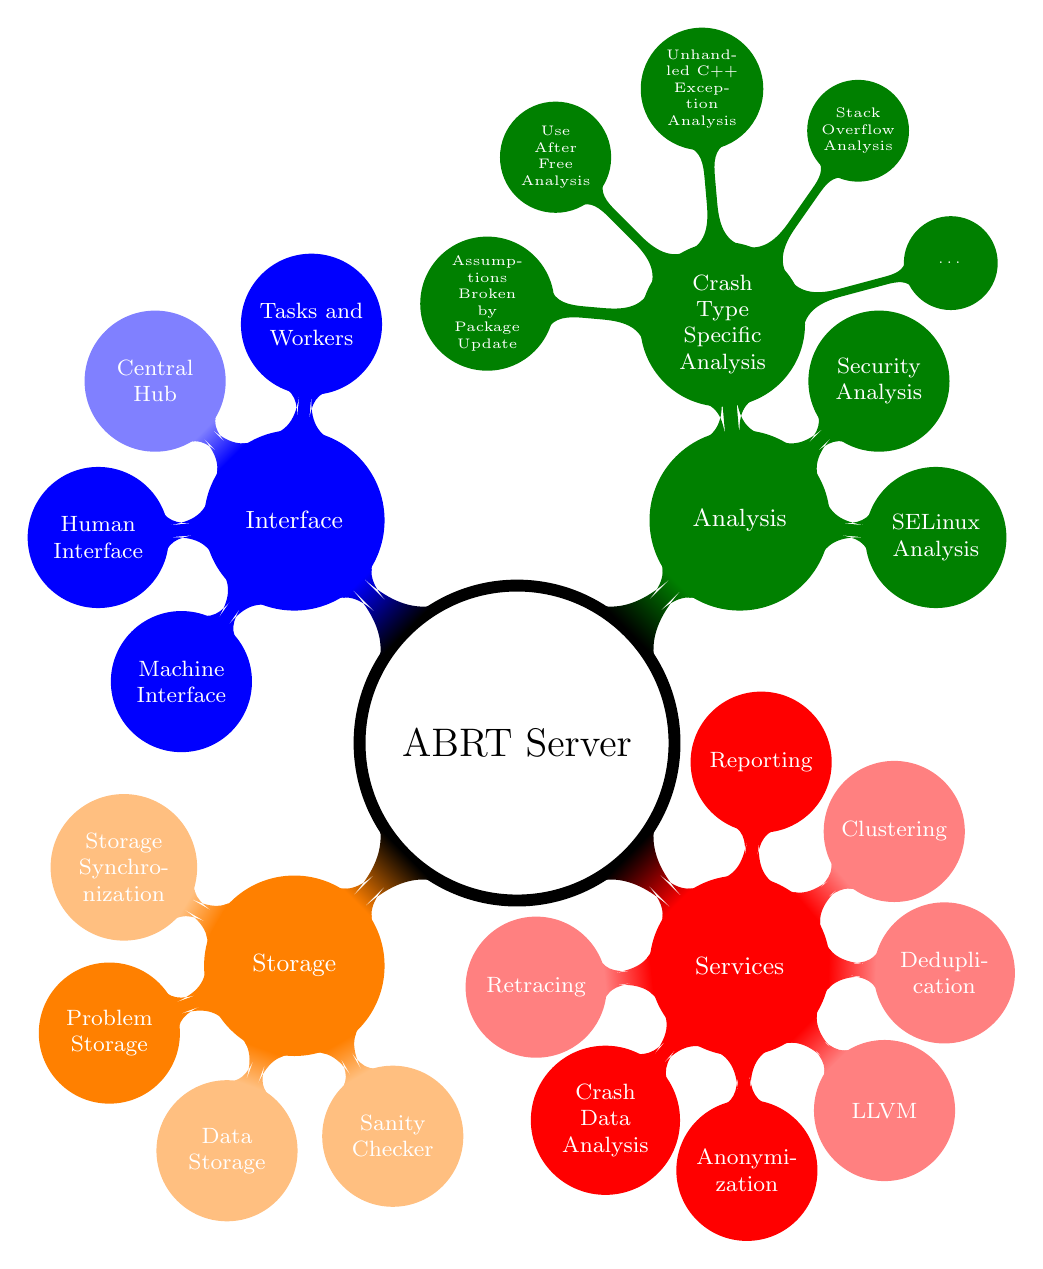
\begin{tikzpicture}[mindmap,
  every node/.style={concept},
  root concept/.append style={concept color=black, fill=white, line width=1ex, text=black, font=\Large},
  text=white,
  storage/.style={concept color=orange, faded/.style={concept color=orange!50}},
  services/.style={concept color=red, faded/.style={concept color=red!50}},
  interface/.style={concept color=blue, faded/.style={concept color=blue!50}},
  analysis/.style={concept color=green!50!black, faded/.style={concept color=green!25!black}},
  grow cyclic,
  level 1/.append style={level distance=4cm, sibling angle=90},
  level 2/.append style={level distance=2.5cm, sibling angle=50},
  level 3/.append style={level distance=3cm, sibling angle=40}]

  \node[root concept] {ABRT Server}
    child[storage] {node {Storage}
      child[faded] {node {Storage Synchronization}}
      child {node {Problem Storage}}
      child[faded] {node {Data Storage}}
      child[faded] {node {Sanity Checker}}
    }
    child[services] {node {Services}
      child[faded, sibling angle=43, level distance=2.6cm] {node {Retracing}}
      child[sibling angle=43, level distance=2.6cm] {node {Crash Data Analysis}}
      child[sibling angle=43, level distance=2.6cm] {node {Anonymi\-zation}}
      child[faded, sibling angle=43, level distance=2.6cm] {node {LLVM}}
      child[faded, sibling angle=43, level distance=2.6cm] {node {Dedupli\-cation}}
      child[faded, sibling angle=43, level distance=2.6cm] {node {Clustering}}
      child[sibling angle=43, level distance=2.6cm] {node {Reporting}}
    }
    child[analysis] {node {Analysis}
      child {node {SELinux Analysis}}
      child {node {Security Analysis}}
      child {node {Crash Type Specific Analysis}
        child {node {\ldots}}
        child {node {Stack Overflow Analysis}}
        child {node {Unhand\-led C++ Exception Analysis}}
        child {node {Use After Free Analysis}}
        child {node {Assump\-tions Broken by Package Update}}
      }
    }
    child[interface] {node {Interface}[clockwise from=100]
      child {node {Machine Interface}}
      child {node {Human Interface}}
      child[faded] {node {Central Hub}}
      child {node {Tasks and Workers}}
    };
\end{tikzpicture}
\end{center}

\begin{description}
\item[Storage] Server's storage is a combination of a database and a
  file server.
  \begin{description}
  \item[Storage Synchronization] Fetches data from external systems,
    such as RPMs and builds from Koji, bugs, comments, attachments
    from Red Hat Bugzilla, components, maintainers, releases from
    Fedora Package Database.
  \item[Problem Storage] We store all issues reported by users
    here. Problems can be program crashes, uncaught Python exceptions,
    Kernel oopses, VM cores, and SELinux denials.
  \item[Data Storage] We download and store RPMs of all versions of
    all packages in operating system.  This is necessary for correct
    retracing of both coredumps and minidumps.  We require both
    binaries and debugging information.  Static analysis requires data
    files from RPMs for greater accuracy.
  \item[Sanity Checker] We measure quality of data (builds, RPMs,
    bugs) downloaded from Fedora Project.  We found quality
    measurement and defect detection to be necessary to keep any
    service operational.  For example, many packages in Fedora and
    RHEL lacked proper debugging information, and this issue blocked
    retracing of many coredumps.  We started to track the quality of
    debugging information and watch for regressions.
  \end{description}
\item[Services] Separate services working on the top of Problem Storage
  and Data Storage. They are triggered by creating a new issue,
  changing the state of the issue, or at a certain time interval.
  \begin{description}
  \item[Retracing] Generates full backtrace from a coredump stored in
    Problem Storage. Generates function names from a minidump
    (coredump-level backtrace) stored in Problem Storage.
  \item[Crash Data Analysis] Depends on Retracing.
  \item[Anonymization] Depends on Crash Data Analysis.
  \item[LLVM] Depends on Anonymization.
  \item[Deduplication] Deduplication happens on several levels:
    minidumps (coredump-level backtraces) are compared when receiving
    a new issue.  Backtraces and/or function names (we call the list
    of function names from the crash thread \textit{optimized
      backtrace} in Faf) are compared when Retracing step is done.
    Analyzed issues are compared when the Crash Type Specific Analysis
    is done.
  \item[Clustering] Clustering finds clusters of issues that are close
    (similar) to each other. Clusters are created fro multiple
    distances. They are used to determine possible components and even
    program functions that are the root cause of the bug.
  \item[Reporting]
  \end{description}
\item[Analysis] Based on static analysis techniques applied to LLVM
  bitcode, the Analysis framework investigates reported issues and
  provide insight at the source code level.
  \begin{description}
  \item[Crash Type Specific Analysis]
  \item[Security Analysis]
  \item[SELinux Analysis]
  \end{description}
\item[Interface] World-facing communication is implemented in the
  web-based Human Interface, and JSON-based Machine Interface.
  Internal interactions between server parts are organized as tasks
  performed by workers. Task queue is managed by central hub, which
  also provides the public communication interfaces.
  \begin{description}
  \item[Human Interface]
  \item[Machine Interface]
  \item[Central Hub]
  \item[Tasks and Workers]
  \end{description}
\end{description}

\subsection{ABRT Server Services Overview}
\begin{center}
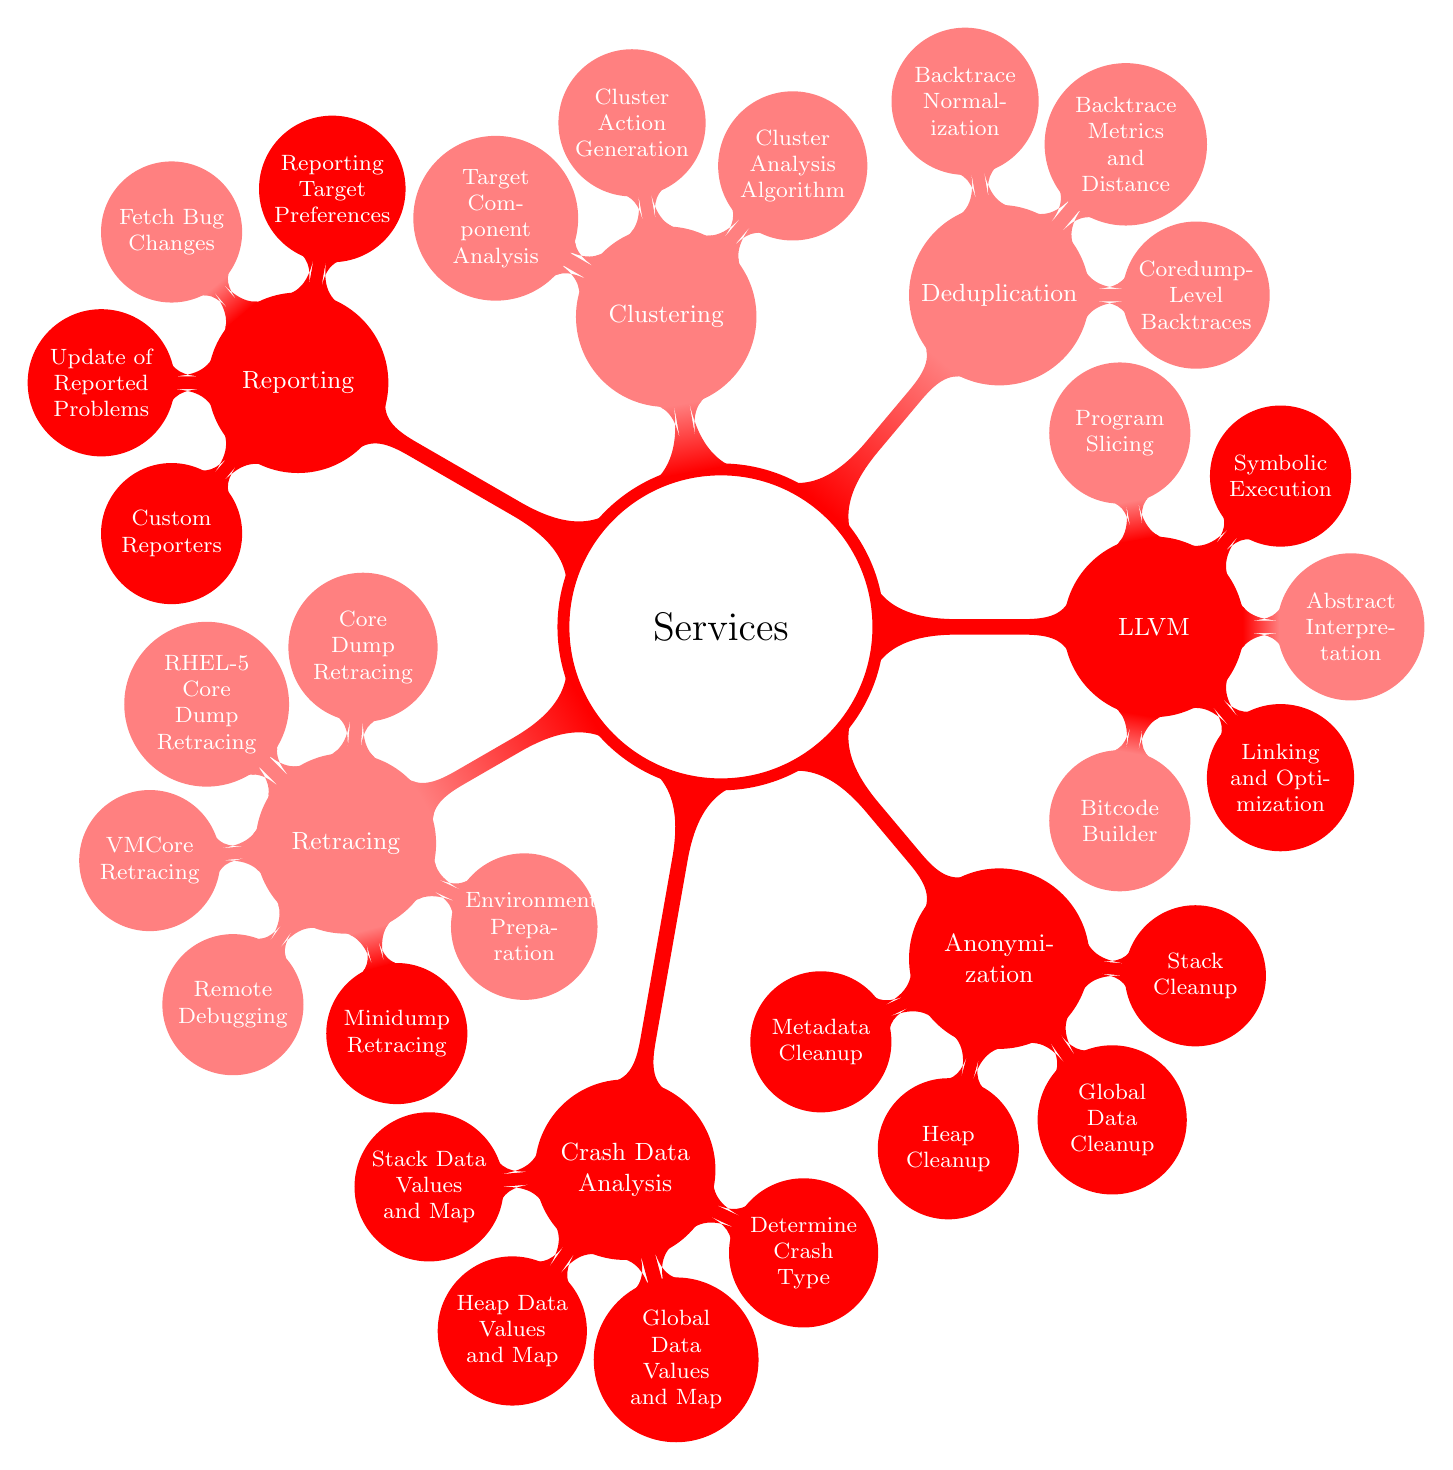
\begin{tikzpicture}[mindmap,
  every node/.style={concept, concept color=red},
  faded/.style={concept color=red!50},
  concept color=red,
  root concept/.append style={fill=white, line width=1ex, text=black, font=\Large},
  text=white,
  grow cyclic,
  level 1/.append style={level distance=5.5cm, sibling angle=50},
  level 2/.append style={level distance=2.5cm, sibling angle=50},
  level 3/.append style={level distance=3cm, sibling angle=40}]
  \node[root concept] {Services}
    child[faded] {node[faded] {Retracing}
      child[faded] {node[faded] {Core Dump Retracing}}
      child[faded] {node[faded] {RHEL-5 Core Dump Retracing}}
      child[faded] {node[faded] {VMCore Retracing}}
      child[faded] {node[faded] {Remote Debugging}}
      child[concept color=red] {node {Minidump Retracing}}
      child[faded] {node[faded] {Environment Preparation}}
    }
    child[level distance=7cm] {node {Crash Data Analysis}
      child {node {Stack Data Values and Map}}
      child {node {Heap Data Values and Map}}
      child {node {Global Data Values and Map}}
      child {node {Determine Crash Type}}
    }
    child {node {Anonymi\-zation}[clockwise from=45]
      child {node {Stack Cleanup}}
      child {node {Global Data Cleanup}}
      child {node {Heap Cleanup}}
      child {node {Metadata Cleanup}}
    }
    child {node {LLVM}
      child[faded] {node[faded] {Bitcode Builder}}
      child {node {Linking and Optimization}}
      child[faded] {node[faded] {Abstract Interpretation}}
      child {node {Symbolic Execution}}
      child[faded] {node[faded] {Program Slicing}}
    }
    child[faded] {node[faded] {Dedupli\-cation}
      child {node[faded] {Coredump-Level Backtraces}}
      child {node[faded] {Backtrace Metrics and Distance}}
      child {node[faded] {Backtrace Normalization}}
    }
    child[faded,level distance=4cm] {node[faded] {Clustering}
      child[faded] {node[faded] {Cluster Analysis Algorithm}}
      child[faded] {node[faded] {Cluster Action Generation}}
      child[faded] {node[faded] {Target Component Analysis}}
    }
    child[level distance=6.2cm] {node {Reporting}[clockwise from=80]
      child {node {Custom Reporters}}
      child {node {Update of Reported Problems}}
      child[faded] {node[faded] {Fetch Bug Changes}}
      child {node {Reporting Target Preferences}}
    };
\end{tikzpicture}
\end{center}

\subsection{ABRT Server Storage Overview}
\begin{center}
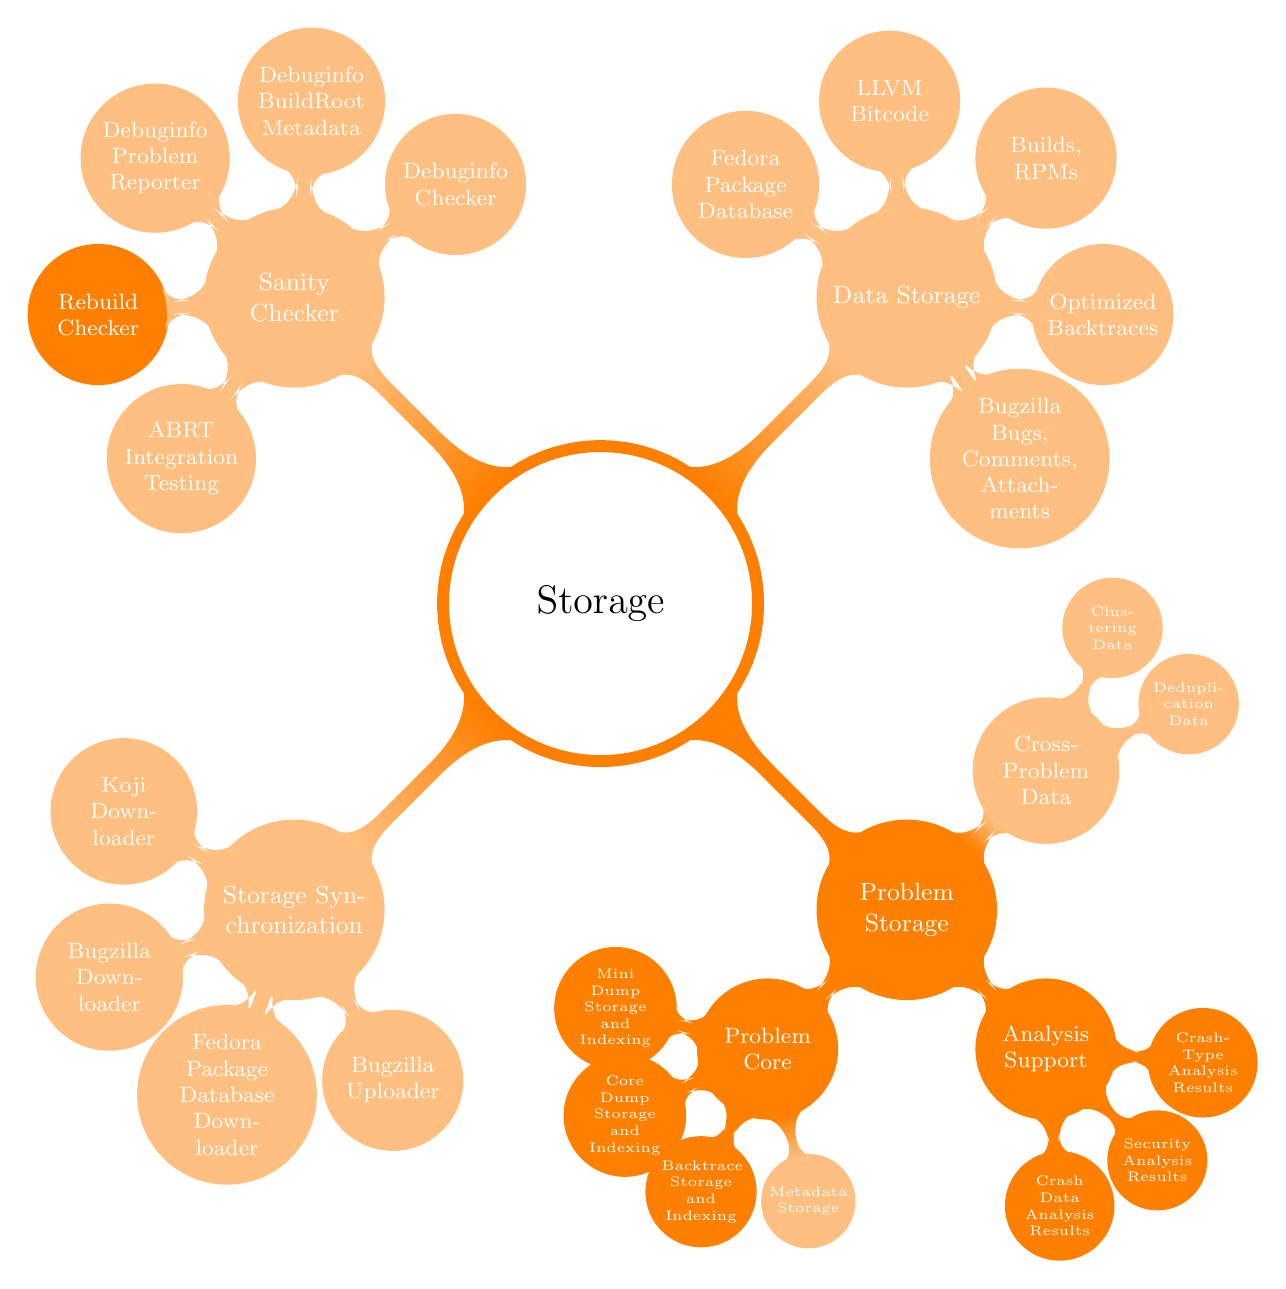
\begin{tikzpicture}[mindmap,
  every node/.style={concept, concept color=orange},
  faded/.style={concept color=orange!50},
  concept color=orange,
  root concept/.append style={fill=white, line width=1ex, text=black, font=\Large},
  text=white,
  grow cyclic,
  level 1/.append style={level distance=5.5cm, sibling angle=90},
  level 2/.append style={level distance=2.5cm, sibling angle=50},
  level 3/.append style={level distance=2cm, sibling angle=40}]
  \node[root concept] {Storage}
    child[faded] {node[faded] {Storage Synchronization}
      child {node[faded] {Koji Downloader}}
      child {node[faded] {Bugzilla Downloader}}
      child {node[faded] {Fedora Package Database Downloader}}
      child {node[faded] {Bugzilla Uploader}}
    }
    child {node {Problem Storage}
      child[sibling angle=90] {node {Problem Core}
        child {node {Mini Dump Storage and Indexing}}
        child {node {Core Dump Storage and Indexing}}
        child {node {Backtrace Storage and Indexing}}
        child[faded] {node[faded] {Metadata Storage}}
      }
      child[sibling angle=90] {node {Analysis Support}
        child {node {Crash Data Analysis Results}}
        child {node {Security Analysis Results}}
        child {node {Crash-Type Analysis Results}}
      }
      child[faded, sibling angle=90] {node[faded] {Cross-Problem Data}
        child[faded] {node[faded] {Dedupli\-cation Data}}
        child[faded] {node[faded] {Clus\-te\-ring Data}}
      }
    }
    child[faded] {node[faded] {Data Storage}
      child {node[faded] {Bugzilla Bugs, Comments, Attachments}}
      child {node[faded] {Optimized Backtraces}}
      child {node[faded] {Builds, RPMs}}
      child {node[faded] {LLVM Bitcode}}
      child {node[faded] {Fedora Package Database}}
    }
    child[faded] {node[faded] {Sanity Checker}
      child[faded] {node[faded] {Debuginfo Checker}}
      child[faded] {node[faded] {Debuginfo BuildRoot Metadata}}
      child[faded] {node[faded] {Debuginfo Problem Reporter}}
      child {node {Rebuild Checker}}
      child[faded] {node[faded] {ABRT Integration Testing}}
    };
\end{tikzpicture}
\end{center}

\subsubsection{Problem Storage}
\begin{center}
\begin{tikzpicture}
\umlclass[x=0,y=0]{problem}{
id : PRIMARY KEY AUTOINCREMENT \\
first occurence : TIMESTAMP \\
last occurence : TIMESTAMP \\
}{}

\umlclass[x=-3,y=-4]{problem report}{
problem id : FOREIGN KEY \\
report id : FOREGIN KEY
}{}

\umlclass[x=3,y=-4]{problem component}{
problem id : FOREIGN KEY \\
component id : FOREGIN KEY \\
order : INT
}{}

\umluniaggreg[geometry=--,pos1=0.2,mult1=1,mult2=+,pos2=0.8]{problem}{problem report}
\umluniaggreg[geometry=--,pos1=0.2,mult1=1,mult2=+,pos2=0.8]{problem}{problem component}

\end{tikzpicture}
\end{center}

\vfill
\subsubsection{Problem Storage -- Reports}

Part of reports is populated from $\mu$reports.

\begin{center}
\scalebox{0.9}{%
\begin{tikzpicture}
\umlclass[x=-2,y=0]{report}{
id : PRIMARY KEY AUTOINCREMENT \\
type : ENUM (USERSPACE, KERNEL, PYTHON, SELINUX) \\
first occurence : TIMESTAMP \\
last occurence : TIMESTAMP \\
crashing component id : FOREIGN KEY
}{}

% Above report left
\umlclass[x=-6,y=3]{report executable}{
report id : PRIMARY KEY \\
path : STRING \\
count : INT
}{}

\umlclass[x=-6,y=6]{report selinux mode}{
report id : FOREIGN KEY \\
selinux mode : ENUM \\
count : INT
}{}

\umlclass[x=-6,y=9]{report selinux context}{
report id : FOREIGN KEY \\
context : STRING NOT NULL \\
count : INT
}{}

\umlclass[x=-6,y=12]{report architecture}{
report id : FOREIGN KEY \\
architecture id : FOREIGN KEY \\
count : INT
}{}

\umluniaggreg[geometry=|-,pos1=0.2,mult1=1,mult2=+,pos2=1.9]{report}{report executable}
\umluniaggreg[geometry=|-,                 mult2=+,pos2=1.9]{report}{report selinux mode}
\umluniaggreg[geometry=|-,                 mult2=+,pos2=1.9]{report}{report selinux context}
\umluniaggreg[geometry=|-,                 mult2=+,pos2=1.9]{report}{report architecture}

% Above report right
\umlclass[x=4,y=3]{report os release}{
report id : FOREIGN KEY \\
operating system release id : FOREIGN KEY \\
count : INT
}{}

\umlclass[x=4,y=9]{report proc status}{
id : PRIMARY KEY \\
report id : FOREIGN KEY \\
traced : BOOL \\
utrace : INT \\
fd size : INT \\
vm peak : INT \\
vm size : INT \\
vm data : INT \\
vm stack : INT \\
vm exe : INT \\
vm lib : INT \\
vm swap : INT \\
threads : INT \\
signal queue : INT \\
signal pending \\
signal block \\
signal ignore \\
...
%capabilities inherited \\
%capabilities prm \\
%capabilities effective \\
%capabilities bnd \\
%cpus allowed \\
%mems allowed \\
%max cpu time \\
%max file size \\
%max data size \\
%max stack size \\
%max core file size \\
%max resident set \\
%max processes \\
%max open files \\
%max locked memory \\
%max address space \\
%max file locks \\
%max pending sygnals \\
%max msgqueue size \\
%max nice priority \\
%max realtime prioriry \\
%max realtime timeout
}{}

\umluniaggreg[geometry=|-,mult2=+,pos2=1.9]{report}{report os release}
\umluniaggreg[geometry=|-,mult2=+,pos2=1.9]{report}{report proc status}

% Below report left
\umlclass[x=-6,y=-4]{report package}{
report id : FOREIGN KEY \\
installed package id : FOREIGN KEY \\
running package id : FOREIGN KEY \\
count : INT
}{}

\umlclass[x=-6,y=-7]{report related package}{
report id : FOREIGN KEY \\
installed package id : FOREIGN KEY \\
running package id : FOREIGN KEY \\
count : INT
}{}

\umluniaggreg[geometry=|-,pos1=0.2,mult1=1,mult2=+,pos2=1.9]{report}{report package}
\umluniaggreg[geometry=|-,                 mult2=+,pos2=1.9]{report}{report related package}

% Below report right
\umlclass[x=7,y=0]{report duplicate hash}{
backtrace id : FOREIGN KEY \\
hash : STRING \\
type : ENUM (NAMES, HASHES)
}{}

\umlclass[x=4,y=-3]{report backtrace}{
id : PRIMARY KEY AUTOINCREMENT \\
report id : FOREIGN KEY
}{}

\umlclass[x=4,y=-6]{report backtrace frame}{
backtrace id : FOREIGN KEY \\
order : INT \\
symbol source id : FOREIGN KEY
}{}

\umluniaggreg[geometry=|-,mult2=+,pos2=1.9]{report}{report backtrace}
\umluniaggreg[geometry=--,mult1=1,mult2=+]{report backtrace}{report backtrace frame}
\umluniaggreg[geometry=--,mult1=1,mult2=+]{report backtrace}{report duplicate hash}

\end{tikzpicture}}
\end{center}

Part of reports is populated from full reports.

\begin{center}
\begin{tikzpicture}
\umlclass[x=-1,y=0]{report}{}{}

% Above report right
\umlclass[x=4,y=3]{report full backtrace}{
id : PRIMARY KEY \\
report id : FOREIGN KEY \\
os release id : FOREIGN KEY \\
text : STRING
}{}

% Above report left
\umlclass[x=-5,y=3]{report coredump}{
id : PRIMARY KEY \\
report id : FOREIGN KEY \\
os release id : FOREIGN KEY
}{}

\umluniaggreg[geometry=|-,mult2=+,pos2=1.9]{report}{report full backtrace}
\umluniaggreg[geometry=|-,mult2=+,pos2=1.9]{report}{report coredump}

\end{tikzpicture}
\end{center}

\subsubsection{Problem Storage -- Report History}
\begin{center}
\begin{tikzpicture}
\umlclass[x=-4,y=0]{report}{}{}

\umlclass[x=5,y=-3]{report history daily}{
day : DATE \\
operating system release id : FOREIGN KEY \\
report id : FOREIGN KEY \\
count : INT
}{}

\umlclass[x=5,y=0]{report history weekly}{
week : DATE \\
operating system release id : FOREIGN KEY \\
report id : FOREIGN KEY \\
count : INT
}{}

\umlclass[x=5,y=3]{report history monthly}{
month : DATE \\
operating system release id : FOREIGN KEY \\
report id : FOREIGN KEY \\
count : INT
}{}

\umluniaggreg[geometry=-|-,pos1=0.2,mult1=1,mult2=*,pos2=1.8]{report}{report history daily}
\umluniaggreg[geometry=--,pos1=0.2,mult2=*,pos2=0.9]{report}{report history weekly}
\umluniaggreg[geometry=-|-,pos1=0.2,mult2=*,pos2=1.8]{report}{report history monthly}

\end{tikzpicture}
\end{center}

\subsubsection{Problem Storage -- Symbols}
\begin{center}
\begin{tikzpicture}
\umlclass[x=0,y=0]{symbol}{
id : PRIMARY KEY \\
name : STRING NOT NULL \\
normalized path : STRING NOT NULL
}{}

\umlclass[x=0,y=-4]{symbol source}{
symbol id : FOREIGN KEY \\
build id : STRING NOT NULL \\
path : STRING NOT NULL \\
offset : INT NOT NULL \\
source file : STRING \\
hash : STRING \\
line number : INT
}{}

\umluniaggreg[geometry=--,pos1=0.2,mult1=1,mult2=+,pos2=0.8]{symbol}{symbol source}

\end{tikzpicture}
\end{center}

\subsection{ABRT Server Interface Overview}
\begin{center}
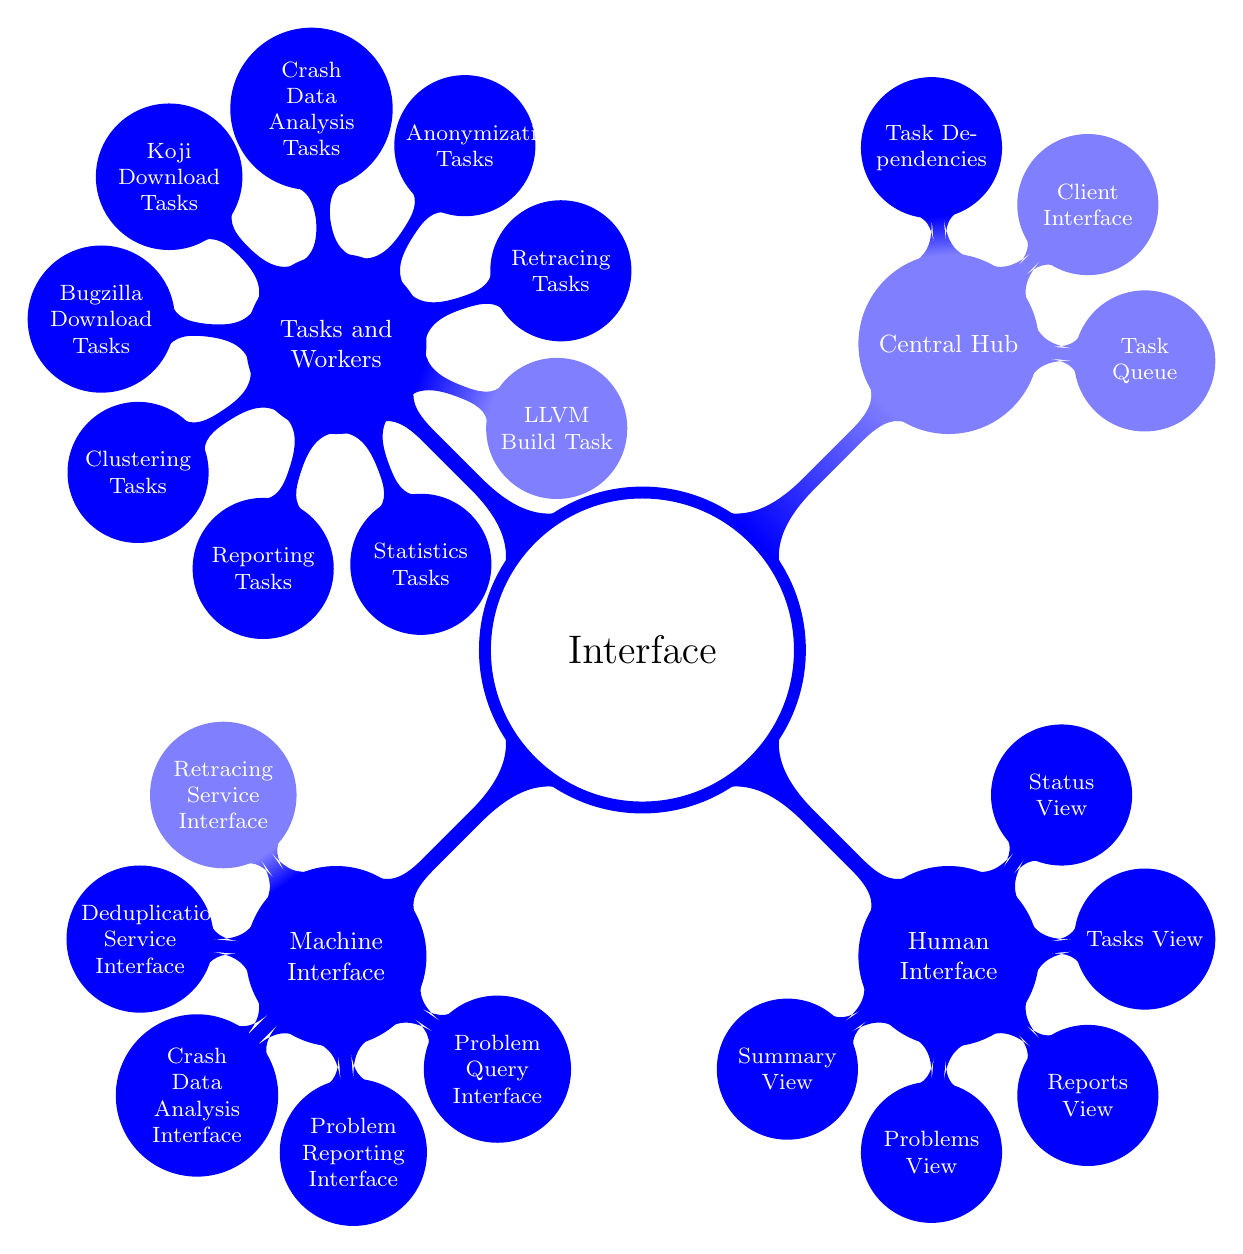
\begin{tikzpicture}[mindmap,
  every node/.style={concept, concept color=blue},
  faded/.style={concept color=blue!50},
  concept color=blue,
  root concept/.append style={fill=white, line width=1ex, text=black, font=\Large},
  text=white,
  grow cyclic,
  level 1/.append style={level distance=5.5cm, sibling angle=90},
  level 2/.append style={level distance=2.5cm, sibling angle=50},
  level 3/.append style={level distance=2cm, sibling angle=40}]
  \node[root concept] {Interface}
    child {node {Machine Interface}
      child[faded] {node[faded] {Retracing Service Interface}}
      child {node {Deduplication Service Interface}}
      child {node {Crash Data Analysis Interface}}
      child {node {Problem Reporting Interface}}
      child {node {Problem Query Interface}}
    }
    child {node {Human Interface}
      child {node {Summary View}}
      child {node {Problems View}}
      child {node {Reports View}}
      child {node {Tasks View}}
      child {node {Status View}}
    }
    child[faded] {node[faded] {Central Hub}
      child {node[faded] {Task Queue}}
      child {node[faded] {Client Interface}}
      child[concept color=blue] {node {Task Dependencies}}
    }
    child {node {Tasks and Workers}
      child[faded, sibling angle=39, level distance=3cm] {node[faded] {LLVM Build Task}}
      child[sibling angle=39, level distance=3cm] {node {Retracing Tasks}}
      child[sibling angle=39, level distance=3cm] {node {Anonymization Tasks}}
      child[sibling angle=39, level distance=3cm] {node {Crash Data Analysis Tasks}}
      child[sibling angle=39, level distance=3cm] {node {Koji Download Tasks}}
      child[sibling angle=39, level distance=3cm] {node {Bugzilla Download Tasks}}
      child[sibling angle=39, level distance=3cm] {node {Clustering Tasks}}
      child[sibling angle=39, level distance=3cm] {node {Reporting Tasks}}
      child[sibling angle=39, level distance=3cm] {node {Statistics Tasks}}
    };
\end{tikzpicture}
\end{center}

\subsubsection{Summary Page}
\begin{center}
\shadowbox{\includegraphics[width=\textwidth, trim=0 3cm 0 0, clip=true]{server-ui-summary.png}}
\end{center}

\begin{description}
\item[Operating System] The available options include Fedora releases,
  pre-release branched Fedora, Fedora Rawhide, All. The list of
  releases should be obtained from Fedora Package Database (this is
  handled by Storage Synchronization.
\item[Components] The available options include All Components, the
  list of all components for the selected Operating System, and
  selected \texttt{comps.xml} groups (such as GNOME Desktop, KDE
  Desktop, Xfce, Web Server, Electronic Lab, Engineering and
  Scientific, Font design and packaging, System Tools, Sound and
  Video, Office/Productivity)
\item[Graph] Displays the number of problems (individual events) in
  time. The underlying data are updated once a day.
\item[Days] The graph shows problems in the last 14 days.
\item[Weeks] The graph shows problems in the last 12 weeks (3 months).
\item[Months] The graph shows problems in the last 12 months.
\item[New and noteworthy] Shows automatically discovered interesting
  trends that can be detected from data.  It tells visitor which
  combinations of Operating System and Component might be worth
  looking.
\end{description}

\subsubsection{Problems Overview Page}
\begin{center}
\shadowbox{\includegraphics[width=\textwidth, trim=0 16cm 0 0, clip=true]{server-ui-problems-overview.png}}
\end{center}

\subsubsection{Problems Item Summary Page}
\begin{center}
\shadowbox{\includegraphics[width=\textwidth, trim=0 5cm 0 0, clip=true]{server-ui-problems-item-summary.png}}
\end{center}

\subsubsection{Reports Overview Page}
\begin{center}
\shadowbox{\includegraphics[width=\textwidth, trim=0 10cm 0 0, clip=true]{server-ui-reports-overview.png}}
\end{center}

\subsubsection{Reports List Page}
\begin{center}
\shadowbox{\includegraphics[width=\textwidth, trim=0 16cm 0 0, clip=true]{server-ui-reports-list.png}}
\end{center}

\subsubsection{Server Tasks Page}
\begin{center}
\shadowbox{\includegraphics[width=\textwidth, trim=0 16cm 0 0, clip=true]{server-ui-tasks.png}}
\end{center}

\subsubsection{Server Status Page}
\begin{center}
\shadowbox{\includegraphics[width=\textwidth, trim=0 17cm 0 0, clip=true]{server-ui-status.png}}
\end{center}

\vfill
\subsubsection{Problem Reporting Interface}

Server accepts microreports.  Microreport is a JSON-formatted data
structure described below:

\begin{center}
\begin{tabular}{l|p{5cm}|c|p{5cm}}
\hline
Name & Format & Mandatory & Notes \\ \hline
\texttt{type} & \texttt{python}, \texttt{userspace}, or \texttt{kerneloops} & yes & \\
\texttt{reason} & Unicode string, max. 128 characters. & yes & Format depends on the \texttt{type}. \\
\texttt{uptime} & Unsigned integer. & yes & Number of seconds from program start to the problem. \\
\texttt{executable} & Full path, max. 512 characters. & yes & \\
\texttt{installed\_package} & Dictionary; see the \texttt{package} table below. & yes & \\
\texttt{running\_package} & Dictionary; see the \texttt{package} table below. & no & \\
\texttt{related\_packages} & List of dictionaries; see the \texttt{related\_package} description below. & yes & \\
\texttt{os} & Dictionary; see the \texttt{os} table below. & yes & \\
\texttt{architecture} & \texttt{x86\_64} or \texttt{i386} & yes & \\
\texttt{reporter} & Dictionary; see the \texttt{reporter} table below. & yes & Program that created the report. \\
\texttt{core\_backtrace} & & yes & \\
\texttt{os\_state} & Dictionary; see the corresponding table below. & yes & \\
\texttt{user\_type} & \texttt{root}, \texttt{nologin}, \texttt{local}, or \texttt{remote} & no & \\
\texttt{selinux} & Dictionary; see the corresponding table below. & no & SELinux presence and mode. \\
\texttt{proc\_status} & ASCII string, max. 2 kB. & & The contents of \texttt{/proc/pid/status}. \\
\hline
\end{tabular}
\end{center}

The \texttt{os} structure:

\begin{center}
\begin{tabular}{l|p{5cm}|c|p{5cm}}
\hline
Name & Format & Mandatory & Notes \\ \hline
\texttt{name} & ASCII string. & yes &  \\
\texttt{version} & ASCII string & yes & Numeric. No codenames. \\
\hline
\end{tabular}
\end{center}

The \texttt{os\_state} structure:

\begin{center}
\begin{tabular}{l|p{5cm}|c|p{5cm}}
\hline
Name & Format & Mandatory & Notes \\ \hline
\texttt{suspend} & \texttt{yes} or \texttt{no} & no & Problem happened during suspend, hibernate, or resume. \\
\texttt{boot} & \texttt{yes} or \texttt{no} & no & Problem happened during boot process. \\
\texttt{login} & \texttt{yes} or \texttt{no} & no & Problem happened during login process. \\
\texttt{logout} & \texttt{yes} or \texttt{no} & no & Problem happened during logout process. \\
\texttt{shutdown} & \texttt{yes} or \texttt{no} & no & Problem happened during the shutdown process. \\
\hline
\end{tabular}
\end{center}

The \texttt{reporter} structure:

\begin{center}
\begin{tabular}{l|p{5cm}|c|p{5cm}}
\hline
Name & Format & Mandatory & Notes \\ \hline
\texttt{name} & ASCII string, max. 128 characters. & yes & \\
\texttt{version} & ASCII string, max. 128 characters. & yes & \\
\hline
\end{tabular}
\end{center}

The \texttt{related\_package} structure:
\begin{center}
\begin{tabular}{l|p{5cm}|c|p{5cm}}
\hline
Name & Format & Mandatory & Notes \\ \hline
\texttt{installed\_package} & Dictionary; see the \texttt{package} table below. & yes & \\
\texttt{running\_package} & Dictionary; see the \texttt{package} table below. & no & \\
\hline
\end{tabular}
\end{center}


The \texttt{package} structure:

\begin{center}
\begin{tabular}{l|p{5cm}|c|p{5cm}}
\hline
Name & Format & Mandatory & Notes \\ \hline
\texttt{name} & ASCII string, max. 128 characters. & yes & \\
\texttt{version} & ASCII string, max. 128 characters. & yes & \\
\texttt{release} & ASCII string, max. 128 characters. & yes & \\
\texttt{architecture} & ASCII string, max. 128 characters. & yes & \\
\texttt{epoch} & ASCII string, max. 128 characters. & yes & \\
\hline
\end{tabular}
\end{center}

The \texttt{selinux} structure:
\begin{center}
\begin{tabular}{l|p{5cm}|p{3cm}|p{5cm}}
\hline
Name & Format & Mandatory & Notes \\ \hline
\texttt{mode} & \texttt{enforcing}, \texttt{permissive}, or \texttt{disabled} & yes & \\
\texttt{context} & ASCII string, max. 128 characters & yes, if the \texttt{mode} is either \texttt{enforcing} or \texttt{permissive} & \texttt{ps -e --context} \\
\texttt{policy\_package} & Dictionary; see the \texttt{package} description. & no & \\
\hline
\end{tabular}
\end{center}


\subsection{ABRT Client Overview}

\begin{center}
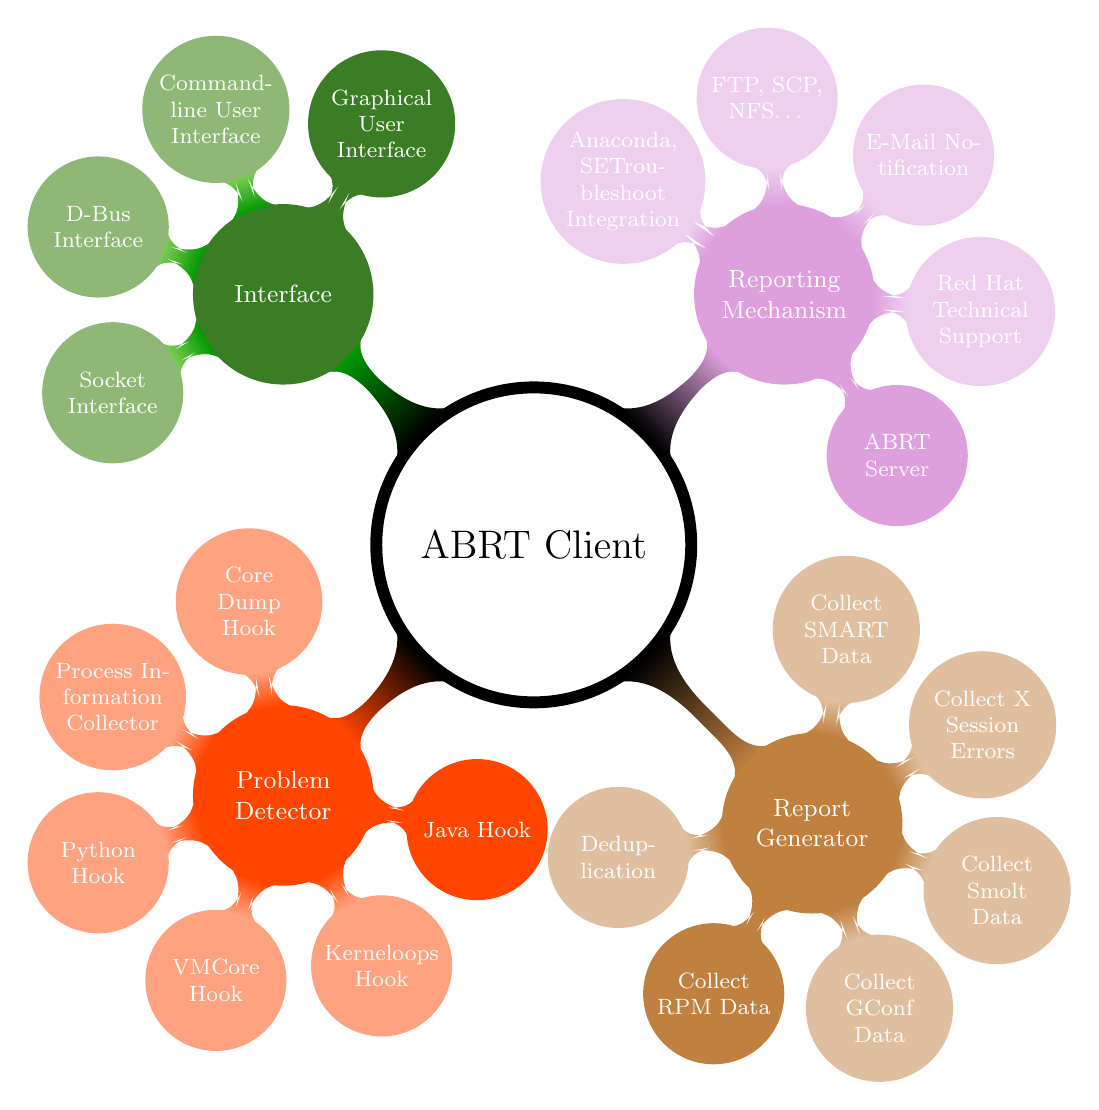
\begin{tikzpicture}[mindmap,
  every node/.style={concept},
  root concept/.append style={concept color=black, fill=white, line width=1ex, text=black, font=\Large},
  text=white,
  detector/.style={concept color=OrangeRed, faded/.style={concept color=OrangeRed!50}},
  generator/.style={concept color=brown, faded/.style={concept color=brown!50}},
  reporting/.style={concept color=Plum, faded/.style={concept color=Plum!50}},
  interface/.style={concept color=OliveGreen, faded/.style={concept color=OliveGreen!50}},
  grow cyclic,
  level 1/.append style={level distance=4.5cm, sibling angle=90},
  level 2/.append style={level distance=2.5cm, sibling angle=50},
  level 3/.append style={level distance=3cm, sibling angle=40}]

  \node[root concept] {ABRT Client}
    child[detector] {node {Problem Detector}
      child[faded] {node[faded] {Core Dump Hook}}
      child[faded] {node[faded] {Process Information Collector}}
      child[faded] {node[faded] {Python Hook}}
      child[faded] {node[faded] {VMCore Hook}}
      child[faded] {node[faded] {Kerneloops Hook}}
      child {node {Java Hook}}
    }
    child[generator, level distance=5cm] {node {Report Generator}
      child[faded] {node[faded] {Dedup\-li\-ca\-tion}}
      child {node {Collect RPM Data}}
      child[faded] {node[faded] {Collect GConf Data}}
      child[faded] {node[faded] {Collect Smolt Data}}
      child[faded] {node[faded] {Collect X Session Errors}}
      child[faded] {node[faded] {Collect SMART Data}}
    }
    child[reporting] {node {Reporting Mechanism}
      child {node {ABRT Server}}
      child[faded] {node[faded] {Red Hat Technical Support}}
      child[faded] {node[faded] {E-Mail Notification}}
      child[faded] {node[faded] {FTP, SCP, NFS\ldots}}
      child[faded] {node[faded] {Anaconda, SETroubleshoot Integration}}
    }
    child[interface] {node {Interface}
      child {node {Graphical User Interface}}
      child[faded] {node[faded] {Command-line User Interface}}
      child[faded] {node[faded] {D-Bus Interface}}
      child[faded] {node[faded] {Socket Interface}}
    };
\end{tikzpicture}
\end{center}

\subsection{ABRT Client Interface Overview}

\begin{center}
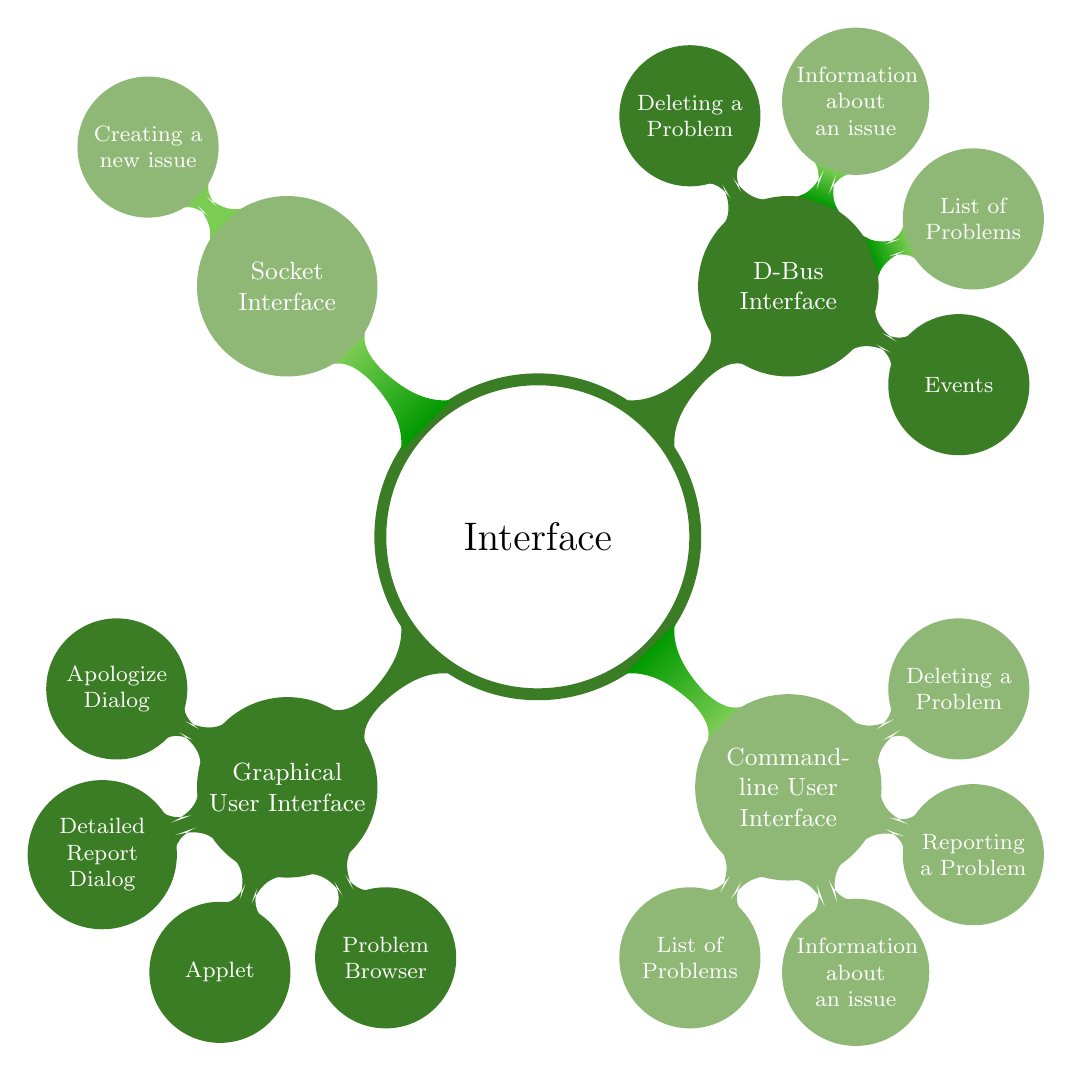
\begin{tikzpicture}[mindmap,
  every node/.style={concept, concept color=OliveGreen},
  faded/.style={concept color=OliveGreen!50},
  concept color=OliveGreen,
  root concept/.append style={fill=white, line width=1ex, text=black, font=\Large},
  text=white,
  grow cyclic,
  level 1/.append style={level distance=4.5cm, sibling angle=90},
  level 2/.append style={level distance=2.5cm, sibling angle=50},
  level 3/.append style={level distance=3cm, sibling angle=40}]

  \node[root concept] {Interface}
    child {node {Graphical User Interface}
      child {node {Apologize Dialog}}
      child {node {Detailed Report Dialog}}
      child {node {Applet}}
      child {node {Problem Browser}}
    }
    child[faded] {node[faded] {Command-line User Interface}
      child {node[faded] {List of Problems}}
      child {node[faded] {Information about an issue}}
      child {node[faded] {Reporting a Problem}}
      child {node[faded] {Deleting a Problem}}
    }
    child {node {D-Bus Interface}
      child {node {Events}}
      child[faded] {node[faded] {List of Problems}}
      child[faded] {node[faded] {Information about an issue}}
      child {node {Deleting a Problem}}
    }
    child[faded] {node[faded] {Socket Interface}
      child[faded] {node[faded] {Creating a new issue}}
    };
\end{tikzpicture}
\end{center}

\cleardoublepage
\subsubsection{Apology Dialog}
The dialogs come from \cite{JonOops}. Please see \cite{JonOops} for
more detailed design.

\begin{center}
\includegraphics[width=\textwidth]{client-ui-apology-dialog-manual.png}
\end{center}

\begin{center}
\includegraphics[width=\textwidth]{client-ui-apology-dialog-automatic.png}
\end{center}

\subsubsection{Detailed Report Dialog}
\begin{center}
\includegraphics[width=\textwidth]{client-ui-detailed-report-dialog.png}
\end{center}

\subsubsection{Applet}

\cleardoublepage
\subsubsection{Problem Browser}
The Problem Browser dialog comes from \cite{JonOops}. Please see
\cite{JonOops} for more detailed design.

\begin{center}
\includegraphics[width=\textwidth]{client-ui-issue-browser.png}
\end{center}

\section{Project Time Management}

\subsection{Fedora 17 Phase}
Finish date: 2012-05-22.

\subsubsection{Sprint 1}
Finish date: 2012-04-20 Friday \\
Duration: 3 weeks

\begin{itemize}
\item Server
  \begin{itemize}
  \item Problem storage
    \begin{itemize}
    \item Database schema [mtoman,mlichvar]
    \item Storage of incoming problems [mlichvar]
    \end{itemize}
  \item Data storage
    \item Initial database schema [mtoman]
  \item Deduplication
    \begin{itemize}
    \item Deduplication of incoming problems according to hashes
    \item Deduplication of retraced problems according to symbols
    \end{itemize}
  \item Retracing
    \begin{itemize}
    \item Retracing of microreports
    \end{itemize}
  \item Machine interface
    \begin{itemize}
    \item Receive report
    \end{itemize}
  \item Migration to SQLAlchemy [mlichvar]
  \item RHEL6 compatibility [mtoman]
  \end{itemize}
\item Client
  \begin{itemize}
  \item Coredump-level backtraces [mmilata]
  \item Microreport sender [npajkovs]
  \item User interface [dvlasenk]
  \end{itemize}
\end{itemize}

\subsubsection{Sprint 2}
Start date: 2012-04-23 Monday \\
Finish date: 2012-05-11 Friday \\
Duration: 3 weeks

\begin{itemize}
\item Server
  \begin{itemize}
  \item Human interface
  \item Machine interface
  \item Tasks and workers
  \item Clustering
    \begin{itemize}
      \item Adapt existing source code to match the server
      \item Properly create problems from reports
    \end{itemize}
  \end{itemize}
\end{itemize}

\subsubsection{Sprint 3}
Start date: 2012-05-14 Monday \\
Finish date: 2012-05-22 Tuesday \\
Duration: 7 days

\subsection{Fedora 18 Phase}
Finish date: 2012-11-01

\subsection{Activity List}

\begin{enumerate}
\item Implement the problem storage tables in SQLAlchemy. [server]
\item Implement server machine interface for communication with client. [server]
\item Implement saving the received microdump to the database. [server]
\item Set-up and document regular, automatic database backup. [server]
\item Finish the design of minireport and fullreport backup. [server]
\item Implement minireport and fullreport backup. [server]
\item Implement deduplication logic on arrival of a new report. [server]
\item Implement deduplication logic for clustering and merging of
  existing reports. [server]
\item Implement coredump-level backtraces. [server]
\item Implement retracing of coredump-level backtraces. [server]
\item Implement the basic layout of human interface. [server]
\item Implement graph on the summary page. [server]
\item Implement initial problems overview page. [server]
\item Implement initial problem summary page. [server]
\item Implement both variants of apology dialog. [client]
\item Implement detailed report dialog. [client]
\item Implement ABRT client uploader. [client]
\item Prepare proposal for Anaconda changes. [client]
\end{enumerate}

- Define Activities
-- Activity List
-- Activity attributes
-- Milestone list

- Sequence Activities
-- Project Schedule Network Diagram

- Estimate Activity Resources
-- Activity Resource Requirements
-- Resource Breakdown Structure

- Estimate Activity Durations
-- Activity Duration Estimates

- Develop Schedule
-- Project Schedule
-- Schedule baseline
-- Schedule data

%\section{Project Cost Management}

%- Estimate Costs
%-- Activity Cost Estimates
%-- Basis of estimates

%- Determine Budget
%-- Cost performance baseline
%-- Project funding requirements

\section{Project Quality Management}

- Plan Quality
-- Quality management plan
-- Quality metrices
-- Quality checklists
-- Process improvement plan

%\section{Project Human Resource Management}

%- Develop Human Resource Plan

%\section{Project Communications Management}

%- Plan Communications

\section{Project Risk Management}

%Plan Risk Management
%-- Risk Register

%Identify Risks

%Perform Qualitative Risk Analysis

%Perform Quantitative Risk Analysis

%Plan Risk Responses

%\section{Project Procurement Management}

%Plan Procurements

%\section{Enterprise Environmental Factors}

%\section{Organizational Process Assets}

\section{Project Management Plan}


\cleardoublepage
\begin{thebibliography}{9}

\bibitem{JonOops}
  Jon McCann,
  \emph{Oops!}.
  \url{https://live.gnome.org/Design/Apps/Oops}.

\bibitem{JonOverview}
  Jon McCann,
  \emph{Problem Recovery and Reporting}.
  \url{https://live.gnome.org/GnomeOS/Design/Whiteboards/ProblemReporting}.

\bibitem{JonProposal}
  Jon McCann,
  \emph{Problem Reporting Architecture Proposal}.
  \url{https://live.gnome.org/GnomeOS/Design/Whiteboards/ProblemReporting/Proposal}.

\bibitem{MS}
  \emph{Debugging in the (Very) Large: Ten Years of Implementation and Experience}.
  \url{http://msdn.microsoft.com/en-us/windows/hardware/gg487440}.

\end{thebibliography}

\end{document}
